% ==========================================================================
% Capítulo: Avances del proyecto
% Estado: se registra en ../STATUS.md, no aquí.
%
% Qué contiene: lo construido hasta la fecha en la prueba de concepto (POC)
% del proyecto, los retos del montaje y cómo se resolvieron, las mediciones
% preliminares y las reuniones de seguimiento. Es un prototipo en un único
% servidor físico; no es el resultado de la evaluación del objetivo 4.
%
% Hechos: ../../project-context/documentation.md, secciones «POC status and
% implementation progress» y «POC sprints and challenges».
% AUTOCONTENIDO: el lector debe entender el capítulo sin consultar el
% repositorio de implementación. No nombrar specs, ADR, dudas, rutas ni
% planes del repositorio (decisión de los autores, 2026-11-07).
% Extensión: unas 3 páginas de texto, más las figuras.
% ==========================================================================
\chapter{Avances del proyecto}\label{cha:avances}

Este capítulo informa el trabajo realizado hasta el 7 de noviembre de 2026 en la prueba de concepto (POC) del proyecto. El prototipo corre en un único servidor físico del laboratorio, sobre el que se simula el clúster con ocho máquinas virtuales, tres de control, tres de servicios y dos de cómputo sin unidad de procesamiento gráfico (GPU), y cada modelo se sirve en un solo nodo de cómputo. El clúster final también tendrá tres nodos de control, alojados en equipos físicos del laboratorio, de modo que el prototipo reproduce esa topología con máquinas virtuales. El POC permite validar el diseño antes de desplegarlo en la sala 104M en diciembre de 2026, y por esa razón su implementación puede cambiar. Las decisiones que aquí se describen son las vigentes a la fecha de corte.

El trabajo del prototipo se desarrolló en dos etapas, entre el 17 de octubre y el 7 de noviembre de 2026, dentro de los \emph{sprints} 2 y 3 del cronograma de la \cref{fig:gantt}. Para validar el diseño de extremo a extremo, el prototipo construyó versiones mínimas de componentes que el cronograma completa en fases posteriores, sin alterar el orden de las fases ni su duración. El \emph{hardware} disponible condicionó el montaje. Sin GPU en el servidor, los motores de inferencia se ejecutan en CPU, lo que limita las mediciones de desempeño a una referencia preliminar, y la validación sobre las GPU de la sala queda para la etapa de despliegue.

\section{Primera etapa: cimientos del clúster}\label{sec:avance-etapa1}

La primera etapa, del 17 al 26 de octubre de 2026, levantó la base sobre la que se construyen los demás componentes. Se montó el servidor y las ocho máquinas virtuales, y sobre ellas se instaló un clúster de Kubernetes con tres nodos de control y una dirección virtual que se mantiene aunque caiga uno de ellos. Sobre ese clúster se desplegaron la entrada fija de la plataforma, la entrega continua desde el repositorio de configuración (GitOps), el cifrado de secretos, el almacenamiento persistente, la base de datos, el registro de imágenes y la observabilidad de métricas y registros. También se activaron las políticas de admisión y el gestor de colas de cómputo, que retiene las cargas que no tienen capacidad disponible. La \cref{fig:poc-montado} muestra el prototipo al cierre de esta etapa.

Durante esta etapa aparecieron tres retos. El primero fue que el sistema operativo de las máquinas virtuales no detectaba el disco ni la red, porque la definición de las máquinas no activaba la interfaz de configuración avanzada y energía con la que el sistema descubre sus dispositivos. Se activó esa interfaz en la definición de las máquinas. El segundo fue que todos los nodos tenían marcas de reserva (\emph{taints}), de modo que los trabajos de instalación de los componentes base no encontraban un nodo donde ejecutarse. Se resolvió dejando los nodos de servicios sin esa marca, identificados solo con una etiqueta. El tercero fue la dependencia de un único nodo de control, cuya caída deja al clúster sin acceso a su interfaz de administración. Los equipos del laboratorio se encienden y se apagan sin aviso, y algunos utilizan discos mecánicos, por lo que ninguno cumple por sí solo la condición de permanecer encendido sin reinicios no anunciados. Por ese motivo el plano de control pasó de uno a tres nodos, de modo que la caída de uno no detenga el clúster, decisión que también se aplica al despliegue en la sala.

\section{Segunda etapa: servicio de modelos y gobierno}\label{sec:avance-etapa2}

La segunda etapa, del 26 de octubre al 7 de noviembre de 2026, construyó el servicio de modelos sobre la base anterior. Cada despliegue se describe como un recurso del clúster que indica el modelo y el motor con que se sirve. La elección del motor depende del formato de los pesos, de modo que los modelos en GGUF se sirven con \emph{llama.cpp} y los modelos en \emph{safetensors} con vLLM. Como línea base, un despliegue se ejecuta como un \emph{Deployment} admitido por la cola de cómputo, y se compara con una variante sobre Ray Serve que usa el mismo motor. En esa variante, un adaptador propio mide el tiempo hasta el primer \emph{token} y la latencia entre \emph{tokens} de cada petición.

Desde el punto de vista de quien usa la plataforma, desplegar un modelo tiene dos momentos. Primero, el administrador da de alta el modelo en el catálogo a partir del identificador de un repositorio externo de modelos. La plataforma muestra una vista previa, descarga los pesos, verifica su integridad y los guarda en el almacén de objetos, y un modelo que está en uso no se puede eliminar. El administrador también otorga a cada usuario el permiso para desplegar. Después, el usuario elige un modelo del catálogo en la interfaz web, selecciona uno de los motores habilitados y, como opción avanzada, el nodo donde quiere ejecutarlo. El estado del despliegue avanza por en cola, admitido, copiando pesos y en ejecución, lo que en el prototipo toma cerca de un minuto, y el modelo queda publicado en una dirección formada por el nombre del usuario y el del despliegue, con una API compatible con OpenAI. Desde la misma interfaz el usuario sigue los registros de su despliegue, lo detiene, lo vuelve a iniciar o lo elimina, mientras el administrador ve y gestiona los despliegues de todos los usuarios.

La \cref{fig:flujo-despliegue} muestra lo que ocurre internamente en ese recorrido. La API verifica que el despliegue quepa en la cuota del usuario y lo registra como un recurso del clúster. El operador observa ese recurso y genera lo que el motor necesita para ejecutarse, que incluye su carga de trabajo, el volumen de pesos y la ruta de red. La cola de cómputo admite la carga o la mantiene en espera hasta que haya cuota, y el planificador la ubica en un nodo de cómputo. Allí, un contenedor de inicio copia los pesos desde el almacén de objetos al volumen del nodo, salvo que ya estén, y el motor los carga y queda disponible en una ruta de la puerta de entrada. La API y el operador se comunican únicamente a través del servidor del clúster, de modo que una solicitud se conserva aunque el operador se detenga.

\begin{figure}[htbp]
  \centering
  \begin{tikzpicture}[
      font=\small,
      paso/.style={draw, rounded corners=2pt, align=center, text width=27mm, minimum height=16mm, font=\footnotesize},
      flecha/.style={-{Stealth[length=2mm]}, semithick},
      etq/.style={font=\scriptsize}]
    \node[paso, fill=black!8] (p1) at (0,0) {\textbf{1. Solicitud}\\El usuario con permiso pide el despliegue desde la web o la API};
    \node[paso] (p2) at (3.6,0) {\textbf{2. API}\\Verifica la cuota y registra el despliegue en el clúster};
    \node[paso] (p3) at (7.2,0) {\textbf{3. Operador}\\Genera la carga del motor, el volumen de pesos y la ruta};
    \node[paso] (p4) at (10.8,0) {\textbf{4. Cola de cómputo}\\Admite la carga si cabe en la cuota del usuario};
    \node[paso] (p5) at (10.8,-3.1) {\textbf{5. Nodo de cómputo}\\Recibe la carga y copia los pesos al volumen};
    \node[paso] (p6) at (7.2,-3.1) {\textbf{6. Motor}\\Carga los pesos y atiende las peticiones};
    \node[paso] (p7) at (3.6,-3.1) {\textbf{7. Puerta de entrada}\\Publica la ruta del modelo};
    \node[paso, fill=black!8] (p8) at (0,-3.1) {\textbf{8. Cliente}\\Consume el modelo con una API compatible con OpenAI};
    \draw[flecha] (p1) -- (p2);
    \draw[flecha] (p2) -- (p3);
    \draw[flecha] (p3) -- (p4);
    \draw[flecha] (p4) -- node[etq, right] {admitida} (p5);
    \draw[flecha] ([xshift=5mm]p4.north) -- ++(0,0.45) -| node[etq, above, pos=0.25] {sin cuota, espera en cola} ([xshift=-5mm]p4.north);
    \draw[flecha] (p5) -- (p6);
    \draw[flecha] (p6) -- (p7);
    \draw[flecha] (p7) -- (p8);
    \node[draw, dashed, align=center, text width=130mm, font=\footnotesize] at (5.4,-5.0)
      {Cada paso deja métricas y registros asociados al usuario y al despliegue, y el estado visible del despliegue avanza por en cola, admitido, copiando pesos y en ejecución};
  \end{tikzpicture}
  \caption[Flujo de un despliegue en el POC]{Flujo de un despliegue en el POC, desde la solicitud del usuario hasta el consumo del modelo. Las flechas indican el orden de los pasos; el paso 4 retiene la carga en cola mientras el usuario no tenga cuota disponible. Elaboración propia.}
  \label{fig:flujo-despliegue}
\end{figure}

Del lado del gobierno, se implementó el operador que traduce las cuotas de cada usuario en un espacio con su límite, y la cuota de la sala en un fondo común que las cuotas individuales pueden usar. Se verificó en el POC que una solicitud que excede la cuota espera en cola, que una carga puede recuperar cuota cuando otra la necesita, y que la carga expropiada queda identificada en su estado. También se verificó que un agotamiento de memoria en un despliegue no afecta a los vecinos, y que las políticas rechazan los despliegues que no cumplen las etiquetas o los límites de la sala.

Los retos de esta etapa fueron de recursos. El servidor del POC tiene 60\,GiB de memoria, así que cada componente declara la memoria y el procesador que solicita y su límite máximo, de modo que la suma se mantiene dentro de la capacidad del servidor. vLLM agotaba la memoria durante su fase de calentamiento, y se resolvió con su modo de ejecución directa (\emph{eager}), que omite ese calentamiento. El escalador automático de Argo CD no tenía solicitudes de memoria con que calcular su uso, y se fijaron esas solicitudes para que el escalado funcione. Por último, la integración con el proveedor institucional de identidad SAAMFI se encuentra en implementación. Mientras tanto, el prototipo usa un proveedor de identidad local que permite probar el flujo de roles, de autenticación y de permisos de extremo a extremo.

Sobre este servicio se construyeron también el importador de pesos, que verifica el tamaño y la integridad de cada archivo antes de registrarlo, la API con usuarios locales y base de datos, una interfaz web mínima, la lectura de registros filtrada por usuario y un panel de métricas por modelo y por despliegue. Los administradores dan de alta los modelos desde la API o desde la interfaz, y la clave de acceso a repositorios externos de modelos se guarda cifrada.

\section{Mediciones preliminares}\label{sec:avance-mediciones}

La \cref{tab:mediciones-poc} recoge las primeras mediciones del POC. Son referencias de funcionamiento en CPU y no constituyen la evaluación de desempeño del \cref{obj:evaluacion}, que aún no se ha ejecutado.

\begin{table}[htbp]
  \centering
  \caption{Mediciones preliminares del POC (solo CPU; no son una evaluación de desempeño).}
  \label{tab:mediciones-poc}
  \begin{tabular}{>{\raggedright\arraybackslash}p{0.44\textwidth} >{\raggedright\arraybackslash}p{0.2\textwidth} >{\raggedright\arraybackslash}p{0.26\textwidth}}
    \toprule
    \textbf{Medición} & \textbf{Resultado} & \textbf{Condición} \\
    \midrule
    \emph{Tokens} por segundo, Qwen3-0.6B en GGUF Q8\_0 con \emph{llama.cpp} & Entre 15 y 17 & 2 CPU por motor \\
    \addlinespace
    \emph{Tokens} por segundo, Qwen3-0.6B con vLLM & Cerca de 3 & 2 CPU \\
    \addlinespace
    Latencia de la variante sobre Ray frente a \emph{llama.cpp} directo & +2,4\,\% & Misma salida y mismas peticiones \\
    \bottomrule
  \end{tabular}
\end{table}

\section{Reuniones de seguimiento}\label{sec:avance-reuniones}

Las reuniones de seguimiento han sido un insumo constante para el alcance y la arquitectura. En las reuniones con el tutor del 26 de agosto y del 9 de septiembre de 2026 se definió que el núcleo del proyecto es la capa de infraestructura y de servicio, que el sistema de cuotas debe gobernar recursos generales y no solo los \emph{tokens} de los modelos de lenguaje, y que los requerimientos se ordenan por prioridad antes de proponer el corte de alcance. En la elicitación con el profesor Alejandro Muñoz Bravo, el 4 de septiembre de 2026, se levantaron las necesidades operativas del laboratorio. Con el profesor Juan Carlos Muñoz, quien dirige el macroproyecto, se acordó que las limitaciones de \emph{hardware} permiten desplegar un modelo por equipo, criterio que el POC adopta. Estas decisiones orientan el diseño que se verifica en el prototipo.

\section{Estado al cierre de la etapa}\label{sec:avance-estado}

Al cierre de la etapa, el prototipo cubre el ciclo de despliegue de un modelo, desde el alta del modelo hasta su consumo por una API compatible con OpenAI, con cuotas, registros y métricas por usuario. Se encuentran en implementación la integración con SAAMFI, la validación de los componentes sobre las GPU de la sala, las reservas por ventana de tiempo y la prioridad por rol, así como los respaldos fuera del clúster. El despliegue en la sala 104M, previsto para diciembre de 2026, incorporará las GPU del laboratorio y permitirá verificar sobre ellas las mediciones de desempeño del \cref{obj:evaluacion}.

\begin{landscape}
\begin{figure}[p]
  \centering
  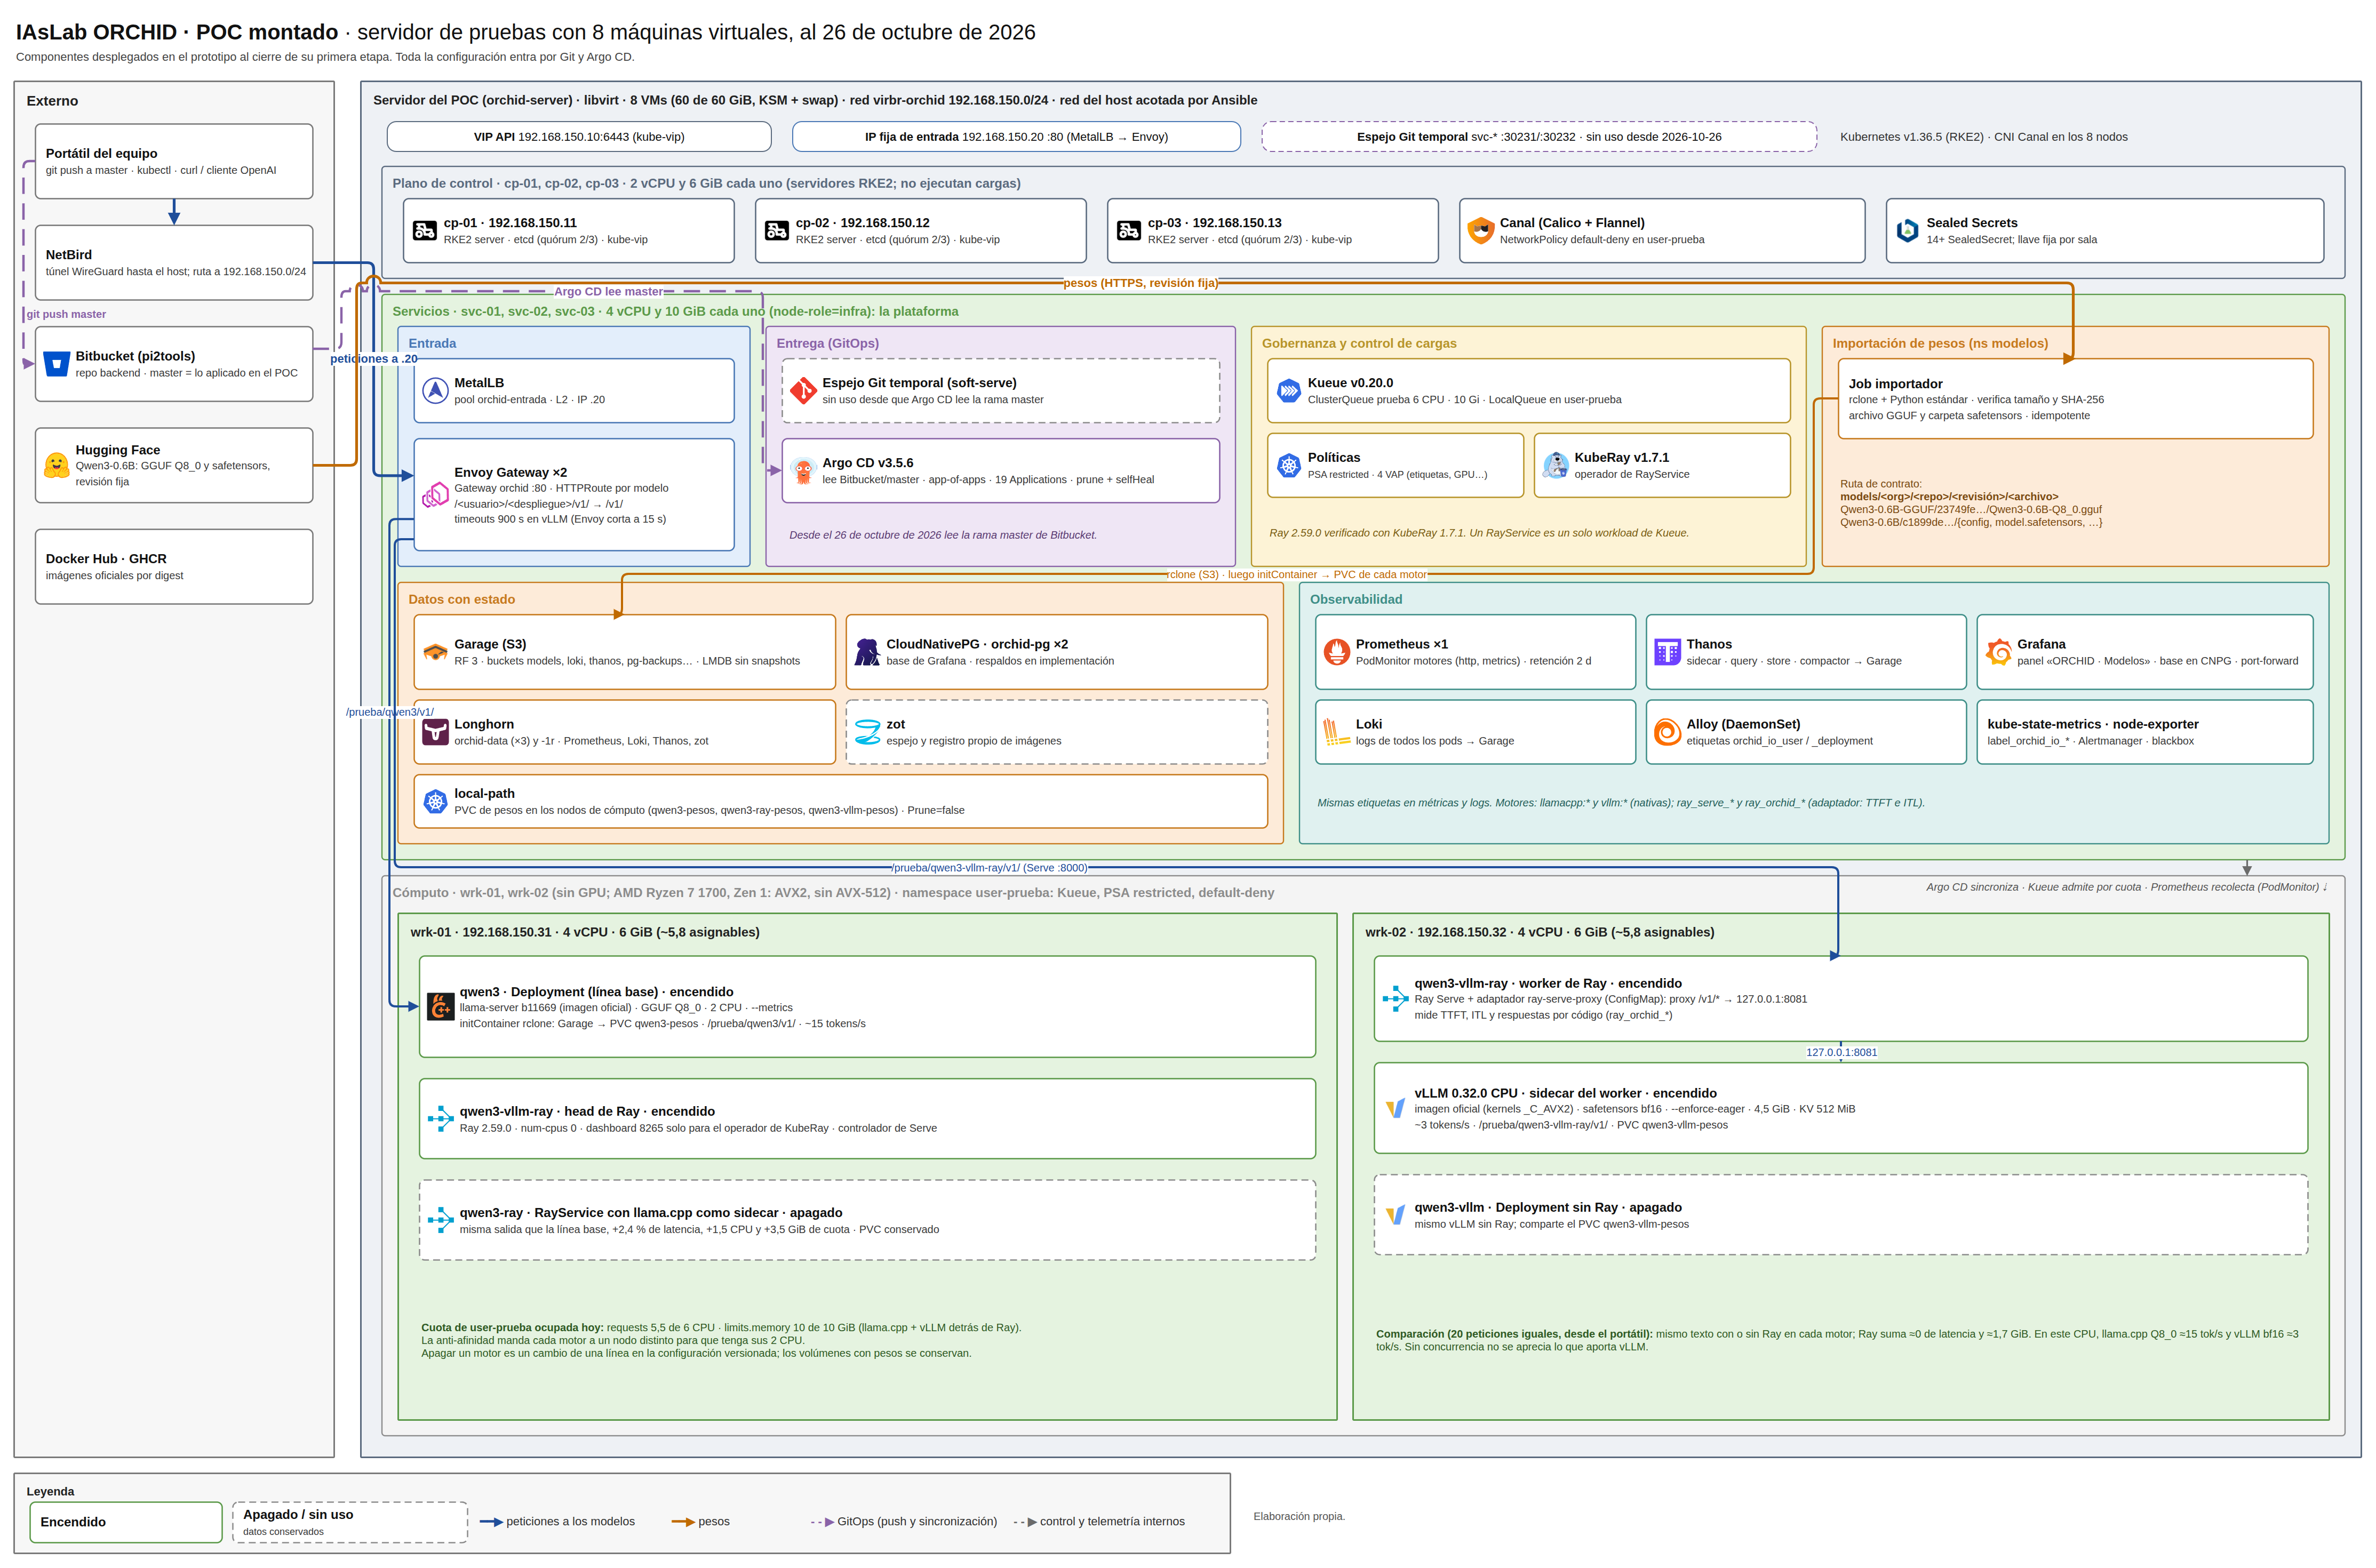
\includegraphics[width=\linewidth]{imagenes/poc-montado.png}
  \caption[Arquitectura del POC al cierre de la primera etapa]{Arquitectura del POC al cierre de la primera etapa, el 26 de octubre de 2026. Muestra los tres nodos de control, los tres nodos de servicios con los componentes de la plataforma y los dos nodos de cómputo sin GPU con los motores en ejecución. Las cajas de borde continuo indican componentes encendidos y las de borde discontinuo, componentes apagados o sin uso. Elaboración propia.}
  \label{fig:poc-montado}
\end{figure}
\end{landscape}
